\section{Analysis Strategy and the \alphat variable}

The goal of the RA1 analysis is to be sensitive to a large a large range of potential DM plus jets models. The guiding principles are low kinematic thresholds, optimised coverage, robustness against systematic effects  and negligible QCD multijet backgrounds contamination. The analysis therefore uses only basic kinematic variables and prefer the used of $H^{miss}_\textrm{T}$ over \etmiss. Because the data taking is also seeded via dedicated trigger utilizing the main kinematic variables kinematic thresholds are as low as:

\begin{itemize}
   \item  $H_\textrm{T}>200$~GeV
   \item  $H^{miss}_\textrm{T}>130$~GeV
   \item  $p_\textrm{T}(j)>40$~GeV
\end{itemize}

The analysis uses the \alphat~\cite{Randall:2008rw, CMS:2008vya, CMS-PAS-SUS-09-001} variable to
 efficiently reject multijet events without significant \met or with transverse energy mismeasurements, 
while retaining a large sensitivity to new physics with final-state signatures containing significant \met.

For dijet events, the \alphat variable is defined as:

\begin{equation}
\label{eq:alphat}
\alphat\, =\, \frac{\Et^{{\rm j}_2}}{M_\text{T}} \, ,
\end{equation}

where $\Et^{\rm j_2}$ is the transverse energy of the less energetic
jet and $M_\text{T}$ is the transverse mass of the dijet system,
defined as

\begin{equation}
  \label{eq:mt}
  M_\text{T}\, = \,\sqrt{ \left( \sum_{i=1}^2 \Et^{{\rm j}_i}
    \right)^2 - \left( \sum_{i=1}^2 p_x^{{\rm j}_i} \right)^2 - \left(
      \sum_{i=1}^2 p_y^{{\rm j}_i} \right)^2} \, .
\end{equation}

where $\Et^{{\rm j}_i}$, $p_x^{{\rm j}_i}$, and $p_y^{{\rm j}_i}$ are,
respectively, the transverse energy and $x$ or $y$ components of the
transverse momentum of jet ${\rm j}_i$.

For a perfectly dijet event with $\Et^{\rm j_1} = \Et^{\rm j_2}$ and back-to-back jets in $\phi$, and in the limit in which the
momentum of each jet is large compared with its mass, the value of \alphat becomes 0.5. If there is an imbalance in the measured
transverse energies of back-to-back jets, \alphat is reduced to a value smaller than 0.5, which gives rise to the variables intrinsic
robustness against jet energy mismeasurements. Values significantly greater than 0.5 are observed when the two jets are not 
back-to-back and are recoiling against significant, genuine \met.

The definition of the \alphat variable can be generalised for events with two or more jets as follows. The mass scale of the physics
processes being probed is characterised by the scalar sum of the transverse energy $\Et$ of jets considered in the analysis, defined as
$\scalht = \sum_{i=1}^{\njet} \Et^{{\rm j}_i}$, where \njet is the number of jets with \Et above a predefined threshold. The estimator
for \met is given by the magnitude of the transverse momenta $\vec{\pt}$ vectorial sum over these jets, defined as $\mht =
|\sum_{i=1}^{N_{\rm jet}} \vec{\pt}^{{\rm j}_i}|$. 

For events with three or more jets, a pseudo-dijet system is formed by combining the jets in the event into two pseudo-jets. The total \Et
for each of the two pseudo-jets is calculated as the scalar sum of the measured \Et of the contributing jets. The combination chosen is the
one that minimises the absolute \Et difference between the two pseudo-jets, \dht. This simple clustering criterion provides the best
separation between multijet events and events with genuine \met. Eq.~\ref{eq:alphat} can therefore be generalised as:

\begin{equation}
  \label{eq:alphat2}
  \alphat\, = \,\frac{1}{2} \times \frac{\scalht -
    \dht}{\sqrt{\scalht^2 - \mht^2}} \, = \,\frac{1}{2} \times 
  \frac{1 - (\dht/\scalht)}{\sqrt{1 - (\mht/\scalht)^2}} \, . 
\end{equation}

In the presence of jet energy mismeasurements, the direction and magnitude of the apparent missing transverse energy, \mht, and energy
imbalance of the pseudo-dijet system, \dht, are highly correlated. This correlation is much weaker for R-parity-conserving SUSY with each
of the two decay chains producing the LSP. It is useful to consider the limiting case $\dht \rightarrow 0$ to
understand the relationship between \alphat and the ratio \mht/\scalht:

\begin{equation}
  \label{eq:alphat3}
  \frac{\mht}{\scalht} \, = \, \sqrt{ 1 - \frac{1}{4 \cdot \alphat^2} }
\end{equation}

For reference, under the assumption of $\dht = 0$, the values of $\alphat = 0.55$, 0.60, and 0.65 map onto values of the ratio
$\mht/\scalht = 0.42$, 0.55, and 0.64. The \alphat is shown in Fig.~\ref{fig:strategy_alphaT}.


\begin{figure}
    \begin{center}
        \subfigure {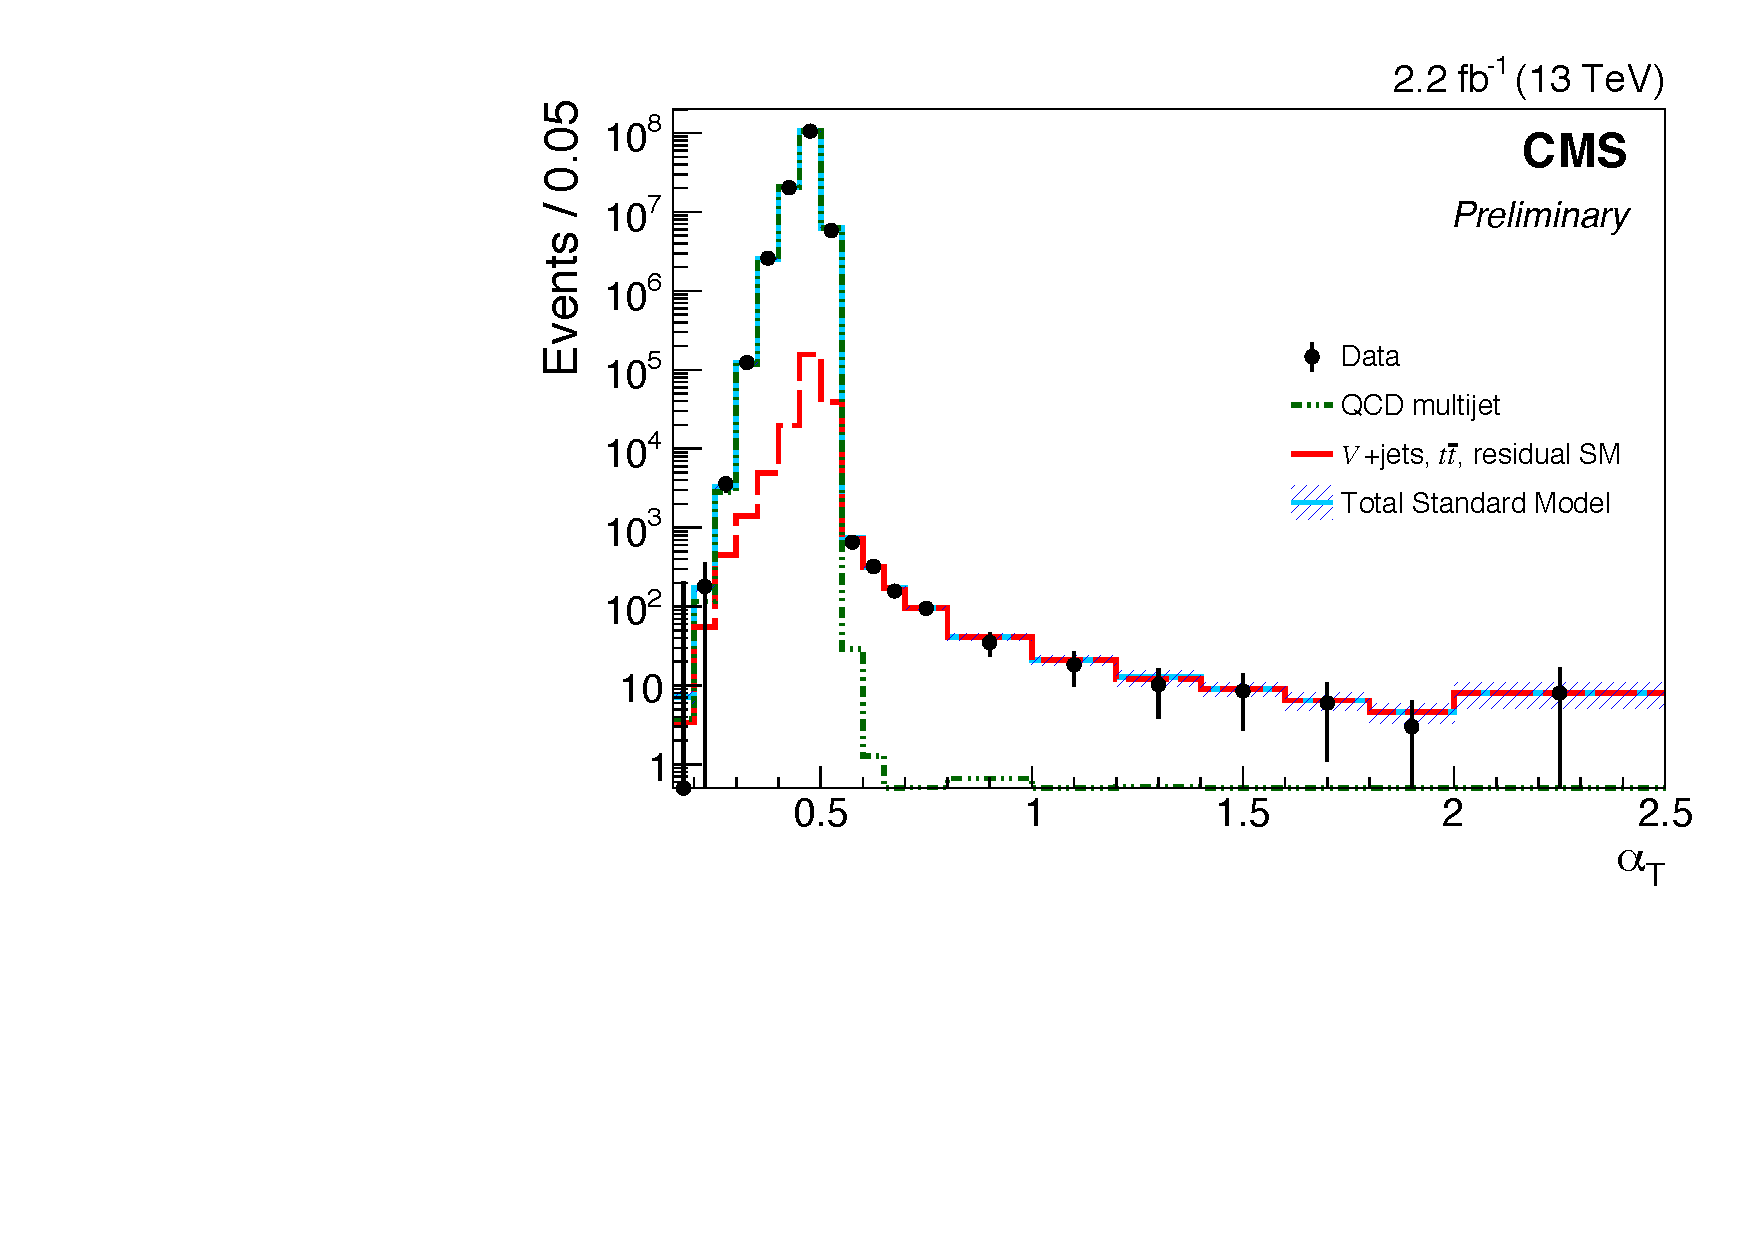
\includegraphics[width=0.5\textwidth]{figures/strategy/alphaT_v4.pdf}} ~~
        \caption{\alphat~variable for the 2015 $13$~TeV data set of $2.2$\ifb}
        \label{fig:strategy_alphaT}
    \end{center}
\end{figure}


Another dedicated variable used is 'biased $\Delta \Phi$' (\bdphi) which is the minimal opening angle between any jet and the \mht vector without considering the tagged jet. This variable is more robust against mis-measurements of the jets compared to the traditional $\temrm{min}\Delta \Phi$ variable and leads to shorter tails as shown in Fig.~\ref{fig:strategy_bdphi}.

 \begin{figure}
    \begin{center}
        \subfigure {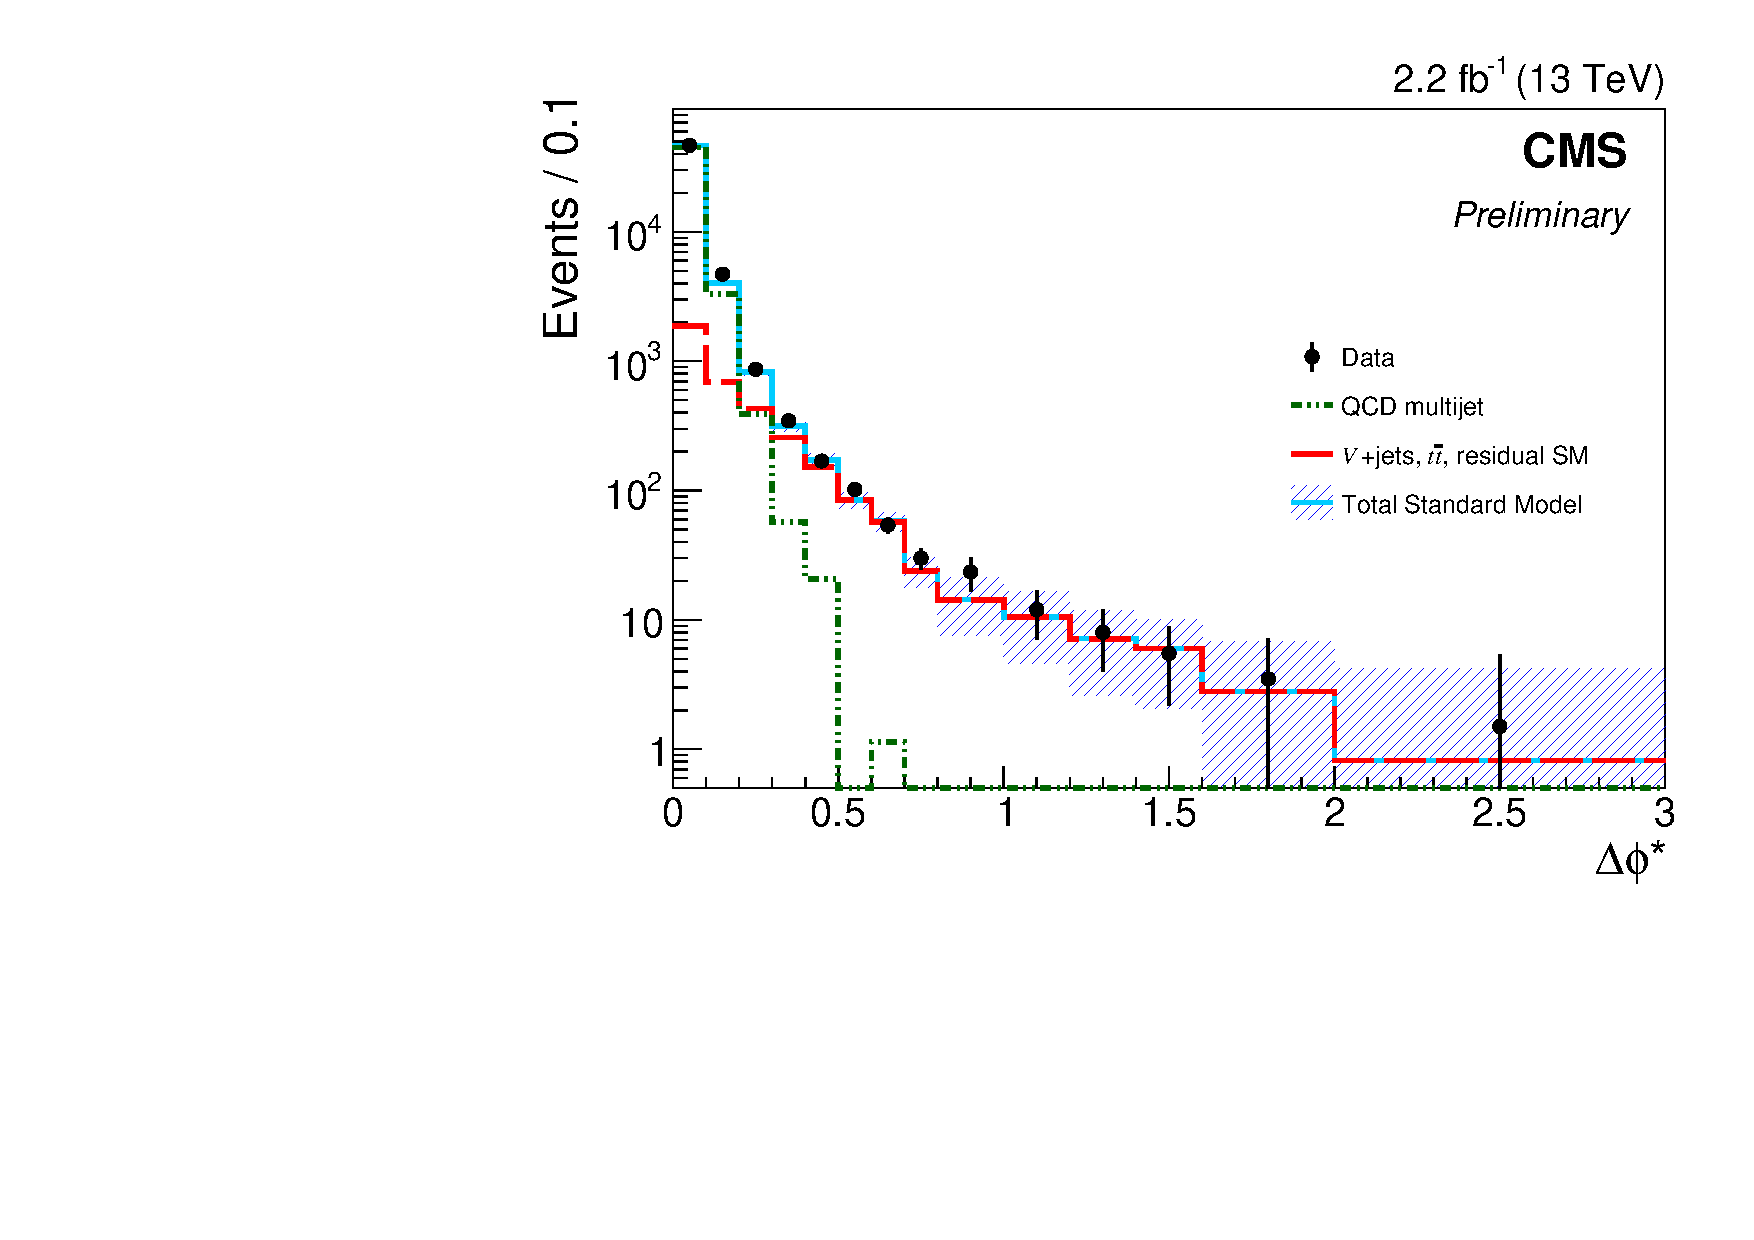
\includegraphics[width=0.5\textwidth]{figures/strategy/bDPhi_v4.pdf}}
        \caption{\bdphi~variable for the 2015 $13$~TeV data set of $2.2$\ifb}
        \label{fig:strategy_bdphi}
    \end{center}
\end{figure}

